% ============================================================
% APRESENTAÇÃO — Curso "Fortalecimento de Lideranças
% Regulatórias Femininas das Comunicações" (ARCTEL 2026)
% Apresentação síncrona, ~5 minutos
% Base visual: _slide/main.tex (paleta e fontes)
% ============================================================

\documentclass[aspectratio=169]{beamer}

% ------------------------------------------------------------
% 1. Pacotes básicos
% ------------------------------------------------------------
\usepackage[T1]{fontenc}
\usepackage[brazilian]{babel}
\usepackage{amsmath,amssymb}
\usepackage{graphicx}
\usepackage{tikz}
\usepackage{xcolor}
\usepackage{booktabs}
\usepackage{array}
\usepackage{multicol}
\usepackage{url}
\usepackage{hyperref}
\usepackage{iftex}

% ------------------------------------------------------------
% 2. Tema visual base
% ------------------------------------------------------------
\usetheme{Madrid}

\ifPDFTeX
  \usepackage[defaultfam,tabular,lining]{montserrat}
  \renewcommand{\familydefault}{\sfdefault}
  \newcommand{\FonteDestaque}{\sffamily\mdseries}
\else
  \usepackage{fontspec}
  \IfFontExistsTF{Montserrat}{%
    \setmainfont{Montserrat}
    \setsansfont{Montserrat}
  }{%
    \IfFontExistsTF{Noto Sans}{%
      \setmainfont{Noto Sans}
      \setsansfont{Noto Sans}
    }{%
      \setmainfont{Latin Modern Sans}
      \setsansfont{Latin Modern Sans}
    }
  }
  \IfFontExistsTF{Ubuntu}{%
    \newfontfamily\UbuntuFont{Ubuntu}
  }{%
    \IfFontExistsTF{Noto Sans}{%
      \newfontfamily\UbuntuFont{Noto Sans}
    }{%
      \newfontfamily\UbuntuFont{Latin Modern Sans}
    }
  }
  \newcommand{\FonteDestaque}{\UbuntuFont\mdseries}
\fi

\usefonttheme{professionalfonts}
\setbeamerfont{normal text}{family=\sffamily}
\setbeamerfont{title}{family=\FonteDestaque,series=\mdseries,size=\LARGE}
\setbeamerfont{subtitle}{family=\FonteDestaque,series=\mdseries,size=\large}
\setbeamerfont{frametitle}{family=\FonteDestaque,series=\mdseries,size=\large}
\setbeamerfont{block title}{family=\FonteDestaque,series=\mdseries}

% ------------------------------------------------------------
% 3. Paleta visual (extraída de assets/css/base/variables.css,
%    a mesma paleta usada em index.html)
% ------------------------------------------------------------
\definecolor{c_verde500}{HTML}{63BF7F}
\definecolor{c_verde600}{HTML}{4BBE6E}
\definecolor{c_verde700}{HTML}{64C080}
\definecolor{c_navy500}{HTML}{497C7E}
\definecolor{c_navy700}{HTML}{275254}
\definecolor{c_white}{HTML}{FFFFFF}
\definecolor{c_black}{HTML}{000000}
\definecolor{c_bgpage}{HTML}{F1F1F1}

\colorlet{ThemePrimary}{c_navy700}
\colorlet{ThemeSecondary}{c_verde600}
\colorlet{ThemeDark}{c_black}
\colorlet{ThemeAccent}{c_verde500}
\colorlet{ThemeAlert}{c_navy500}
\colorlet{ThemeLight}{c_bgpage}

\setbeamercolor{normal text}{fg=ThemeDark,bg=ThemeLight}
\setbeamercolor{background canvas}{bg=ThemeLight}
\setbeamercolor{palette primary}{bg=ThemePrimary, fg=ThemeLight}
\setbeamercolor{palette secondary}{bg=ThemeSecondary, fg=ThemeLight}
\setbeamercolor{palette tertiary}{bg=ThemeDark, fg=ThemeLight}
\setbeamercolor{palette quaternary}{bg=ThemeAlert, fg=ThemeLight}
\setbeamercolor{frametitle}{bg=ThemePrimary, fg=ThemeLight}
\setbeamercolor{title}{fg=ThemeLight}
\setbeamercolor{subtitle}{fg=ThemeAccent}
\setbeamercolor{author}{fg=ThemeLight}
\setbeamercolor{institute}{fg=ThemeLight}
\setbeamercolor{date}{fg=ThemeLight}
\setbeamercolor{structure}{fg=ThemeSecondary}
\setbeamercolor{alerted text}{fg=ThemeAlert}
\setbeamercolor{block title}{bg=ThemeSecondary, fg=ThemeLight}
\setbeamercolor{block body}{bg=ThemeLight, fg=ThemeDark}
\setbeamercolor{itemize item}{fg=ThemeAccent}
\setbeamercolor{itemize subitem}{fg=ThemeSecondary}
\setbeamercolor{section in toc}{fg=ThemePrimary}

\setbeamertemplate{navigation symbols}{}

% ------------------------------------------------------------
% 4. Logo no canto superior direito
% ------------------------------------------------------------
\newcommand{\logounb}{../assets/img/logo/logo-unb.png}

\addtobeamertemplate{frametitle}{}{%
    \begin{tikzpicture}[remember picture,overlay]
        \node[anchor=north east, xshift=-0.25cm, yshift=0cm]
            at (current page.north east)
            {\IfFileExists{\logounb}{\includegraphics[height=0.65cm]{\logounb}}{}};
    \end{tikzpicture}
}

\graphicspath{{./}}

% ------------------------------------------------------------
% 5. Metadados
% ------------------------------------------------------------
\title[ARCTEL 2026]{Fortalecimento de Lideranças Regulatórias\\Femininas das Comunicações}
\subtitle{Apresentação do Curso}
\author[Coordenação ARCTEL]{Coordenação do Curso}
\institute[UnB]{Universidade de Brasília}
\date{2026}

% ============================================================
\begin{document}

% ------------------------------------------------------------
% CAPA
% ------------------------------------------------------------
\begin{frame}
  \titlepage
\end{frame}

% ------------------------------------------------------------
\begin{frame}{Coordenação}
\centering
\vspace{0.5em}
\begin{columns}[T,onlytextwidth]
\column{0.33\textwidth}
\centering
\textbf{Luis Fernando\\Ramos Molinaro}\\[0.5em]
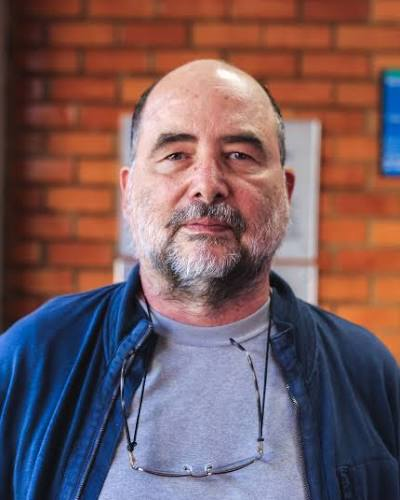
\includegraphics[width=0.55\linewidth]{img/luis.jpg}
\column{0.33\textwidth}
\centering
\textbf{Paulo Henrique \\Portela de Carvalho}\\[0.5em]
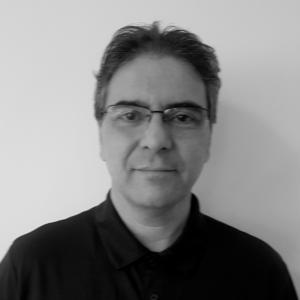
\includegraphics[width=0.55\linewidth]{img/paulo.png}
\column{0.33\textwidth}
\centering
\textbf{Marcio Nunes Iorio \\Aranha Oliveira}\\[0.5em]
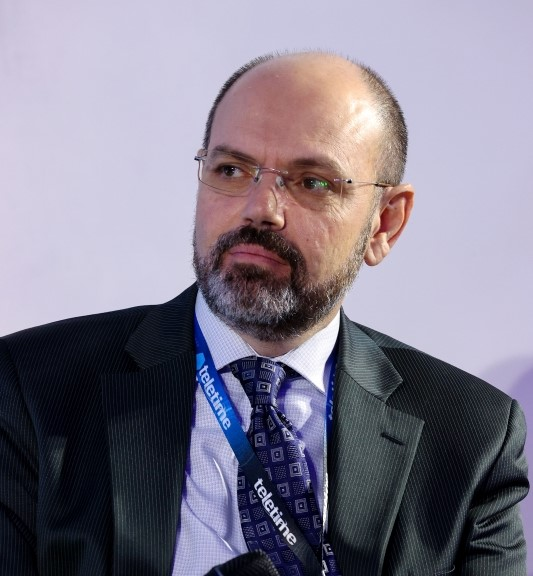
\includegraphics[width=0.55\linewidth]{img/marcio.jpg}
\end{columns}
\end{frame}

% ------------------------------------------------------------
\begin{frame}{Curso: módulos e calendário}
\small
\begin{itemize}
  \item \textbf{11 módulos}, carga total de \textbf{60 horas}
  \item Modalidade: \textbf{online síncrona}
  \item Período: \textbf{04/08/2026} até \textbf{final de novembro/2026}
  \item Ritmo: terças e quintas, \textbf{8h–10h} (horário de Brasília)
  \begin{itemize}
    \item quarta-feira, mesmo horário, como alternativa de contingência
  \end{itemize}
  \item Ementas, professores e referências: detalhados no site do curso
\end{itemize}
\end{frame}

% ------------------------------------------------------------
\begin{frame}{Horários de cada país}
\small
\centering
\renewcommand{\arraystretch}{1.25}
\begin{tabular}{lcc}
\toprule
\textbf{País} & \textbf{Fuso} & \textbf{8h Brasília =} \\
\midrule
Brasil (Brasília)          & UTC$-3$      & 08h \\
Cabo Verde                 & UTC$-1$      & 10h \\
Guiné-Bissau / São Tomé     & UTC$+0$      & 11h \\
Portugal (continental)     & UTC$+0/+1$   & 11h (12h no verão) \\
Angola / Guiné Equatorial  & UTC$+1$      & 12h \\
Moçambique                 & UTC$+2$      & 13h \\
Timor-Leste                & UTC$+9$      & 20h \\
\bottomrule
\end{tabular}

\vspace{0.6em}
\footnotesize Portugal é o único país da CPLP com horário de verão (29/03 a 25/10/2026).
\end{frame}

% ------------------------------------------------------------
\begin{frame}{Perfil dos professores}
\centering
\vspace{-0.3em}
\tiny
\begin{columns}[T,onlytextwidth]
\column{0.33\textwidth}
\centering
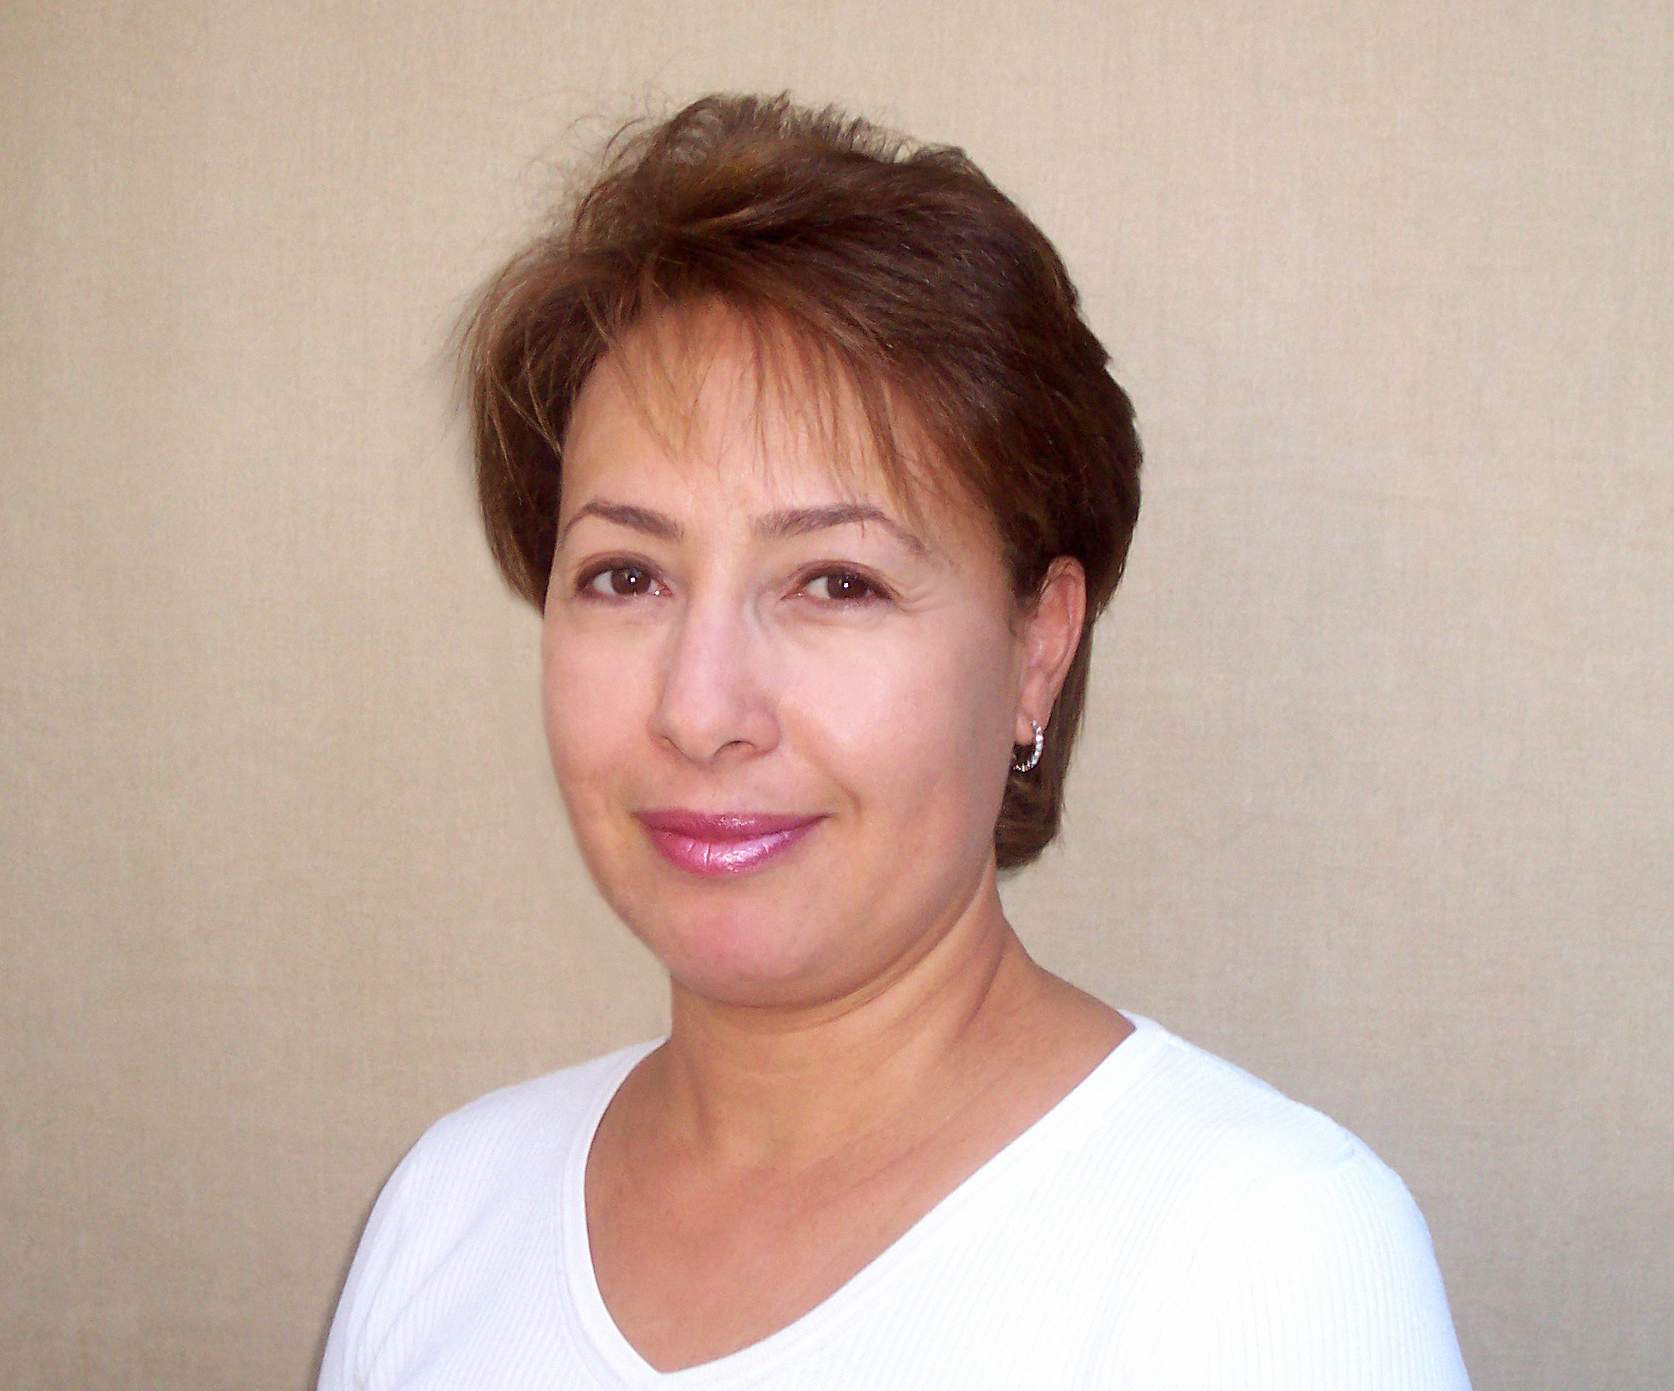
\includegraphics[height=1.9cm]{img/professores/NeliaDelBianco.png}\\[0.15em]
\textbf{Nélia Del Bianco}\\
Comunicação (jornalismo, mídia)
\column{0.33\textwidth}
\centering
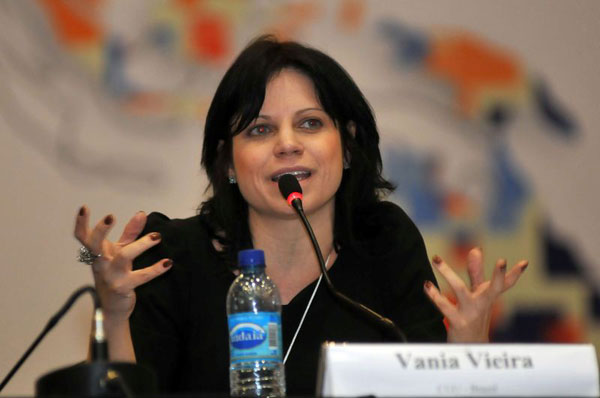
\includegraphics[height=1.9cm]{img/professores/VaniaLuciaRibeiroVieira.jpg}\\[0.15em]
\textbf{Vânia Lúcia Ribeiro Vieira}\\
Direito Administrativo/Regulatório
\column{0.33\textwidth}
\centering
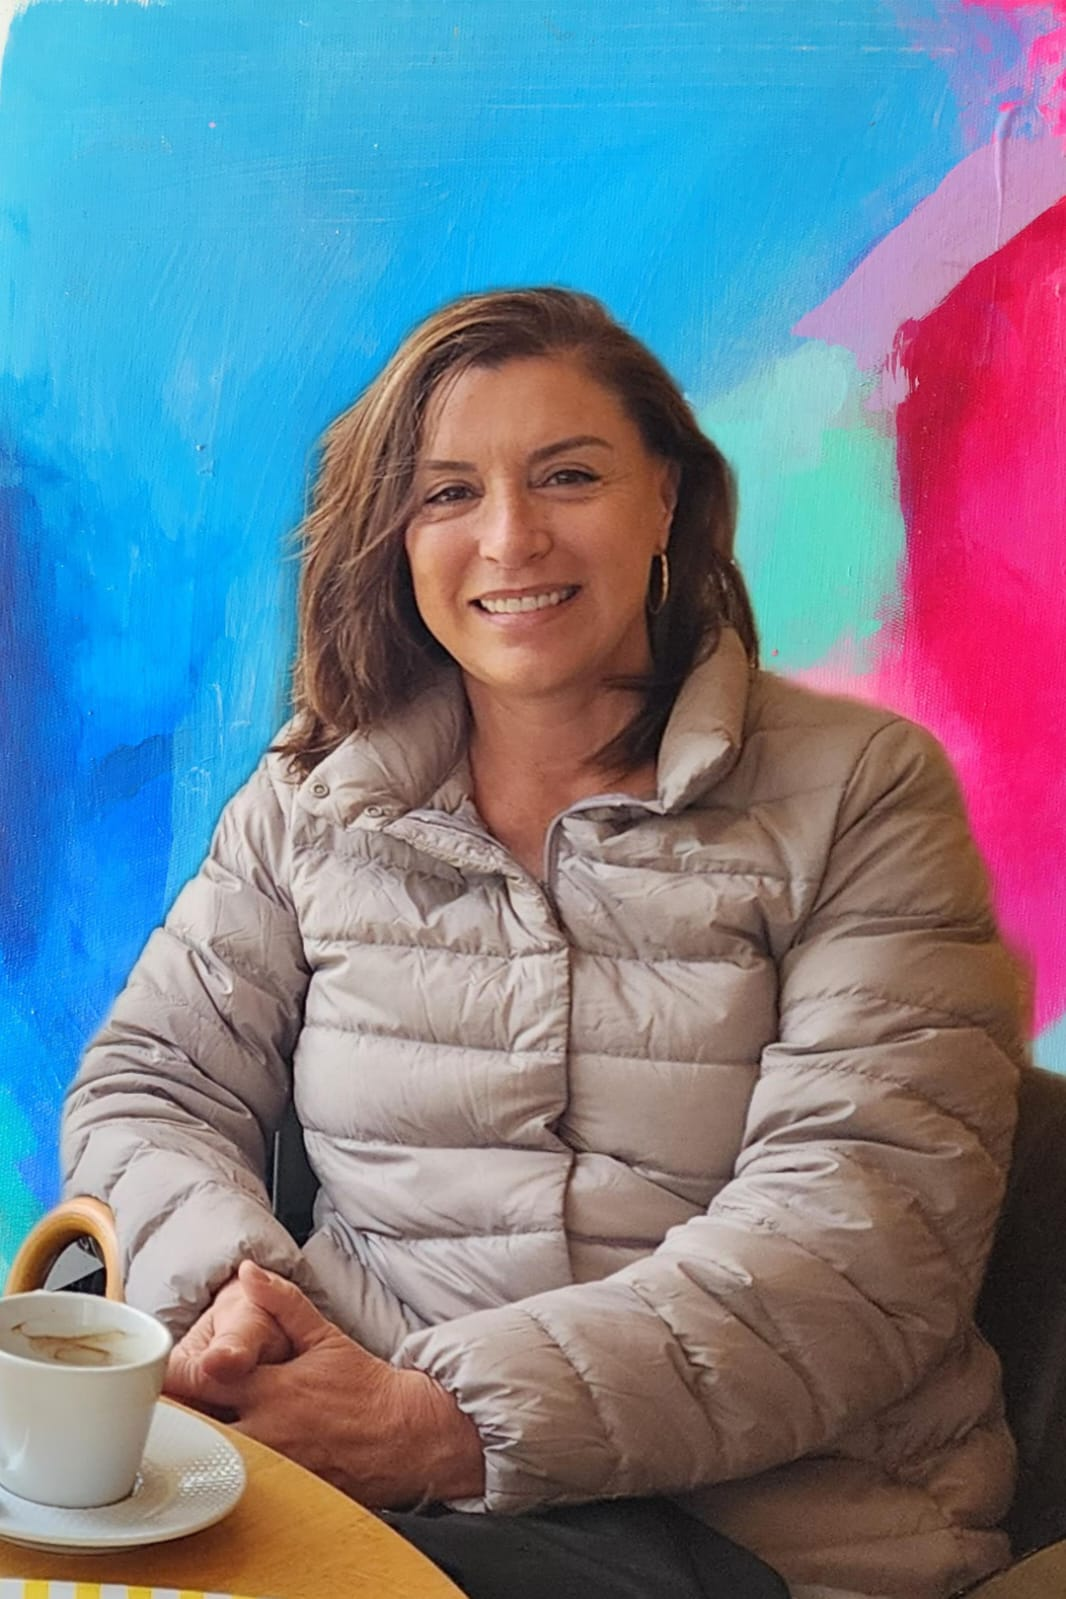
\includegraphics[height=1.9cm]{img/professores/SimoneHenriquetaCossetinScholze.jpeg}\\[0.15em]
\textbf{Simone H. Cossetin Scholze}\\
Direito, C\&T
\end{columns}

\vspace{0.35em}
\begin{columns}[T,onlytextwidth]
\column{0.33\textwidth}
\centering

\includegraphics[height=1.9cm]{img/professores/BrunoRamosFernandes.png}\\[0.15em]
\textbf{Bruno Ramos Fernandes}\\
Ciências Contábeis, tributação
\column{0.33\textwidth}
\centering
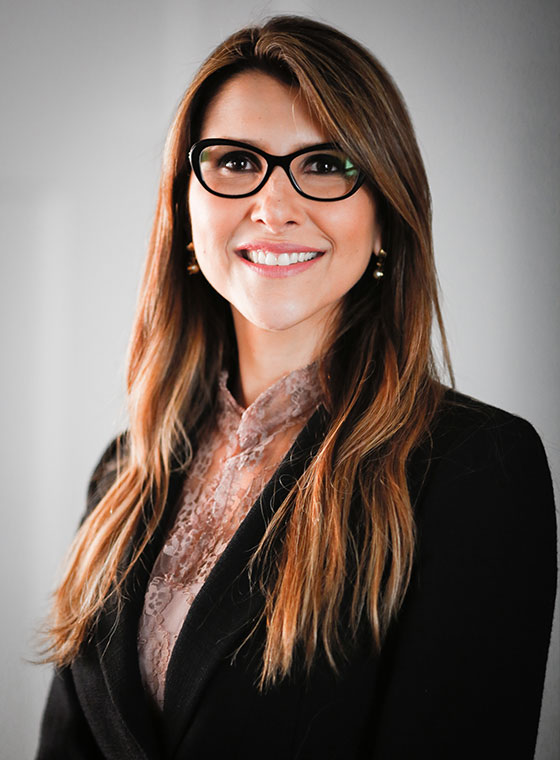
\includegraphics[height=1.9cm]{img/professores/AnadeOliveiraFrazaoVieiradeMello.jpg}\\[0.15em]
\textbf{Ana Frazão Vieira de Mello}\\
Direito Civil/Econômico, ex-CADE
\column{0.33\textwidth}
\centering
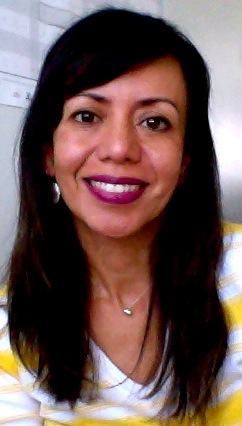
\includegraphics[height=1.9cm]{img/professores/PriscilaAmericaSolisMendezBarreto.png}\\[0.15em]
\textbf{Priscila América Solís Mendez Barreto}\\
Engenharia Elétrica/Computação
\end{columns}
\end{frame}

% ------------------------------------------------------------
\begin{frame}{Operacionalização das aulas}
\small
\begin{itemize}
  \item Curso síncrono via \textbf{Teams}
  \item Aulas online, ao vivo, duas vezes por semana
  \item Aulas gravadas e disponibilizadas \textbf{no site} do curso e na Plataforma Microsoft Teams
  \item Slides e materiais de referência disponibilizados por módulo
  \item Quem falta: \textbf{atividade substitutiva} (questionário sobre o conteúdo — compensa frequência)
\end{itemize}
\end{frame}

% ------------------------------------------------------------
\begin{frame}{Site do curso — central de informação}
\small
\begin{columns}[T,onlytextwidth]
\column{0.28\textwidth}
\centering
\textbf{Site do curso}\\[0.4em]

\includegraphics[width=0.85\linewidth]{qrcode/site.png}\\[0.4em]
{\small\url{nmi-unb.github.io/arctel2026/}}
\column{0.72\textwidth}
\begin{itemize}
  \item \textbf{Início} — visão geral do curso
  \item \textbf{Módulos} — ementa, professor, referência e link da aula
  \item \textbf{Próximas aulas}
  \item \textbf{Calendário} — cronograma completo
  \item \textbf{Avisos} — comunicados
  \item \textbf{Contato} — canal oficial
\end{itemize}
\end{columns}
\end{frame}

% ------------------------------------------------------------
\begin{frame}{Avaliação}
\small
\begin{itemize}
  \item Frequência mínima: \textbf{75\%}
  \item Estudo de caso individual ou em grupo, alinhado a um dos módulos
  \item Entrega em até 30 dias após o término do último módulo
  \item Aprovação = frequência + estudo de caso
\end{itemize}
\end{frame}

% ------------------------------------------------------------
\begin{frame}{Canais de Contato}
\centering
\begin{columns}[T,onlytextwidth]
\column{0.33\textwidth}
\centering

\includegraphics[width=0.6\linewidth]{qrcode/whatsApp.png}\\[0.3em]
\small Grupo WhatsApp
\column{0.33\textwidth}
\centering
\vspace{1cm}
\small\textbf{arctel2026@ccom.unb.br}\\[0.8em]
\small\textbf{+55 61 3107 5656}
\column{0.33\textwidth}
\centering

\includegraphics[width=0.6\linewidth]{img/leonardo.png}\\[0.3em]
\small Leonardo Botelho
\end{columns}

\vspace{1em}
\small Todo assunto do curso deve passar por esses canais e pelo site
\end{frame}

\end{document}
